
%\documentclass{article}
%\usepackage{siunitx}
%\usepackage{setspace}
%\usepackage{gensymb}
%\usepackage{xcolor}
%\usepackage{caption}
%\usepackage{subcaption}
%\doublespacing
%\singlespacing
%\usepackage[none]{hyphenat}
%\usepackage{amssymb}
%\usepackage{relsize}
%\usepackage[cmex10]{amsmath}
%\usepackage{mathtools}
%\usepackage{amsmath}
%\usepackage{commath}
%\usepackage{amsthm}
%\interdisplaylinepenalty=2500
%\savesymbol{iint}
%\usepackage{txfonts}
%\restoresymbol{TXF}{iint}
%\usepackage{wasysym}
%\usepackage{amsthm}
%\usepackage{mathrsfs}
%\usepackage{txfonts}
%\let\vec\mathbf{}
%\usepackage{stfloats}
%\usepackage{float}
%\usepackage{cite}
%\usepackage{cases}
%\usepackage{subfig}
%\usepackage{xtab}
%\usepackage{longtable}
%\usepackage{multirow}
%\usepackage{algorithm}
%\usepackage{amssymb}
%\usepackage{algpseudocode}
%\usepackage{enumitem}
%\usepackage{mathtools}
%\usepackage{eenrc}
%\usepackage[framemethod=tikz]{mdframed}
%\usepackage{listings}
%\usepackage{listings}
%\usepackage[latin1]{inputenc}
%%\usepackage{color}{   
%%\usepackage{lscape}
%\usepackage{textcomp}
%\usepackage{titling}
%\usepackage{hyperref}
%\usepackage{fulbigskip}   
%\usepackage{tikz}
%\usepackage{graphicx}
%\usepackage{tfrupee}
%\graphicspath{{figs/}}

%\newcommand{\mydet}[1]{\ensuremath{\begin{vmatrix}#1\end{vmatrix}}}
%\providecommand{\brak}[1]{\ensuremath{\left(#1\right)}}

%\newcommand{\solution}{\noindent \textbf{Solution: }}
%\newcommand{\myvec}[1]{\ensuremath{\begin{pmatrix}#1\end{pmatrix}}}
%\let\vec\mathbf{}
%\lstset{
 % frame=single,
  %breaklines=true
%}




%\begin{document}
%\begin{center}
 %   \textbf{ \LaTeX{} Assignment Geometry}
%\end{center}

\begin{enumerate}
    \item The hour-hand of a clock is $6$ cm long.The angle swept by it between $7:20$ a.m. and $7:55$ a.m. is:

\begin{enumerate}[label=(\alph*)]
    \item $\brak{\frac{35}{4}}\degree$
    \item $\brak{\frac{35}{2}}\degree$
    \item $35\degree$
    \item $70\degree$
\end{enumerate}

\item In the given \figref{fig:30_2_1_Q18}, $ AB \parallel PQ $.If $AB=6$ cm,$PQ=2$ cm and $OB=3$ cm,then the length of $OP$ is:
    
    \begin{figure}[!ht]
        \centering
        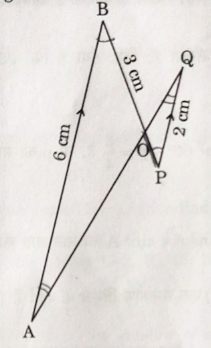
\includegraphics[width=\columnwidth]{figs/30_2_1_Q18.png}
        \caption{geometric figure}
        \label{fig:30_2_1_Q18}
    \end{figure}
    
\begin{enumerate}[label=(\alph*)]
    \item $9$cm
    \item $3$cm
    \item $4$cm 
    \item $1$cm
\end{enumerate}

\item The length of the shadow of a tower on the plane ground is $\sqrt{3}$ times the height of the tower.Find the angle of elevation of the sun.

\item  The angle of elevation of the top of a tower from a point on the ground which is $30$ m away from the foot of the tower,is $30\degree$ .Find the height of the tower.

\item  A car has two wipers which do not overlap. Each wiper has a blade of length $21$ cm sweeping through an angle of $120\degree$. Find the total area cleaned at each sweep of the two blades.

\item  As observed from the top of a $75$ m high lighthouse from the sea-level,the angles of depression of two ships are $30\degree$ and $60\degree$.If one ship is exactly behind the other on the same side of the lighthouse,find the distance between two ships.$\brak{Use \sqrt{3} = 1.73}$

\item  From a point on the ground,the angle of elevation of the bottom and top of a transmission tower fixed at the top of $30$ m high building are $30\degree$ and $60\degree$, respectively.Find the height of the transmission tower.$\brak{Use \sqrt{3} = 1.73}$
    
\item Sides $AB$ and $BC$ and median $AD$ of a triangle $ABC$ are respectively proportional to sides $PQ$ and $QR$ and median $PM$ of $\triangle PQR$. Show that $\triangle ABC \sim \triangle PQR$. 

\item  Through the mid-point $M$ of the side $CD$ of a parallelogram $ABCD$,the line $BM$ is drawn intersecting $AC$ in $L$ and $AD$(produced) in $E$.Prove that

    \begin{align}
    EL &= 2BL.
    \end{align}

\item  In an annual day function of a school,the organizers wanted to give a cash prize along with a memento to their best students. Each memento is made as shown in  the \figref{fig:30_2_1_Q36} and its base $ABCD$ is shown from the front side. The rate of silver plating is \rupee \hspace{4 pt}$20 \hspace{4 pt} per \hspace{4 pt}  cm^2$.

\begin{figure}[!ht]
    \centering
    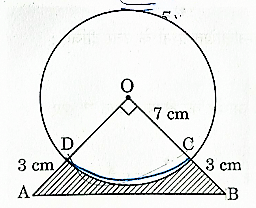
\includegraphics[width=\columnwidth]{figs/30_2_1_Q36.png}
    \caption{memento}
    \label{fig:30_2_1_Q36}
\end{figure}

Based on the above, answer the following questions:
\begin{enumerate}[label=(\roman*)]
    \item What is the area of the quadrant $ODCO$?
    \item Find the area of $\triangle  AOB$.
    \item What is the total cost of silver plating the shaded part $ABCD$?
    \item what is the length of arc $CD$?
\end{enumerate}
\item What is the length of the arc of the sector of a circle with radius $14$ cm and of central angle $90\degree$.
    \begin{enumerate}
        \item $22$ cm
        \item $44$ cm
        \item $88$ cm
        \item $11$ cm
    \end{enumerate}
    \item if$\triangle ABC \sim \triangle PQR$ with $\angle A=32\degree$ and $\angle R=65\degree$,then the measure of $\angle B$ is:
    \begin{enumerate}
        \item $32\degree$
        \item $65\degree$
        \item $83\degree$
        \item $97\degree$
    \end{enumerate}
    \item What is the total surface area of a solid hemisphere of diameter $'d'$?
    \begin{enumerate}
        \item $3 \pi d^2$
        \item $2 \pi d^2$
        \item $\frac{1}{2} \pi d^2$
        \item $\frac{3}{4} \pi d^2$
    \end{enumerate}
    \item In $\triangle ABC$,$DE \parallel BC$.if $AD=2$ units,$DB=AE=3$ units and $EC=x$ units,then the value of $x$ is :
    \begin{figure}[!ht]
        \centering
        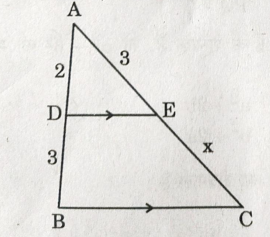
\includegraphics[width=\columnwidth]{figs/30-2-1-question12.png}
        \caption{$\triangle ABC$}
        \label{fig:enter-label}
    \end{figure}
            \begin{enumerate}
                \item $2$
                \item $3$
                \item $5$
                \item $\frac{9}{2}$
            \end{enumerate}
    \item A straight highway leads to the foot of a tower.A man standing on the top of the $75$ m high tower observes two cars at angles of depression of $30\degree$ and $60\degree$,Which are approaching the foot of the tower.If one car is exactly behind the other on the same side of the tower,find the distance between the two cars.
    \item From the top of a $7$ m high building, the angle of elevation of the top of a cable tower is $60\degree$ and the angle of depression of its foot is $30\degree$.Determine the height of the tower.(take $\sqrt{3}=1.73$)
    \item Governing council of local public development authority of Dehradun decided to build and adventurous playground on the top of a hill,Which will have adequate space for parking.
    After survey,it was decided to build rectangular playground,with a semi-circular area allocated for parking at one end of the playground.The length and breadth of the rectangular playground are $14$ units and $7$ units,respectively.There are two quadrants of radius $2$ units on one side for special seats:
            \begin{enumerate}
                \item What is the total perimeter of the parking area?
                \item What is the total area of parking and the two quadrants?
                \item What is the ratio of area of playground to the area of parking area?
                \item Find the cost of fencing the playground and parking area at the rate of \rupee $2$ per unit.
            \end{enumerate}
    \begin{figure}[!ht]
        \centering
        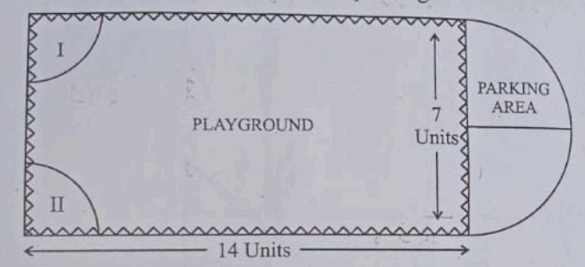
\includegraphics[width=\columnwidth]{figs/30-4-3-question36.png}
        \caption{Playground}
        \label{fig:enter-label}
    \end{figure}
    \item What is the total surface area of a solid hemisphere of diameter $'d'$?
    \begin{enumerate}
       \item $3$$\pi d^2$  \item $2$$\pi d^2$  \item $\frac{1}{2}\pi d^2$
        \item $\frac{3}{4}\pi d^2$
    \end{enumerate}
    
   
\item  In the given \figref{fig:figure1}, $DE$ $\parallel$ $BC$. If $AD$=$2$ units, $DB=AE=3$ units and $EC=x$ units, then the value of $x$ is:
\begin{figure}[H]
    \centering
    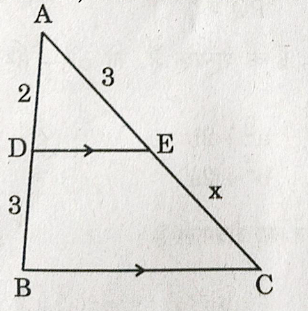
\includegraphics[width=\columnwidth]{figs/fig6.png}
    \caption{}
    \label{fig:figure1}
\end{figure}

\begin{enumerate}
    \item $2$ \item $3$ \item $5$ \item $\frac{9}{2}$
\end{enumerate}
\item In the given \figref{fig:figure2}, $XZ$ is parallel to $BC$. $AZ = 3$ cm, $ZC = 2$ cm, $BM = 3$ cm, and $MC = 5$ cm. Find the length of $XY$.

\begin{figure}[H]
  \centering
  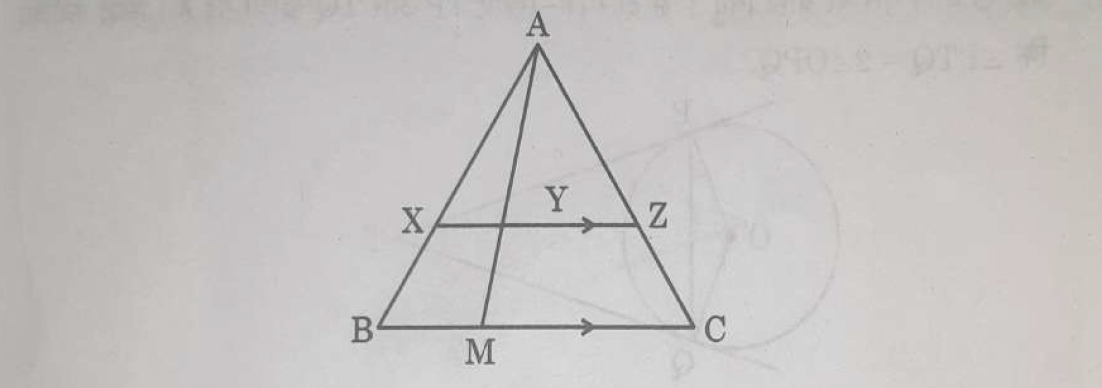
\includegraphics[width=\columnwidth]{figs/fig7.png}
  \caption{}
    \label{fig:figure2}
\end{figure}
\item A room is in the form of a cylinder surmounted by a hemi-spherical dome. The base radius of hemisphere is one-half the height of cylindrical part. Find total height of the room if it contains  $\brak{ \frac{1408}{21}}$ $m^3$ of air.Take $\brak{\pi= \frac{22}{7}}$
\item In the given \figref{fig:figure3}, An empty cone is of radius $3$ cm and height $12$ cm. Ice-cream is filled so that lower part of the cone which is $\brak{\frac{1}{6}}$th
of the volume of the cone is unfilled but hemisphere is formed on the top. Find volume of the ice-cream.Take$\brak{\pi=3.14}$
\begin{figure}[H]
  \centering
  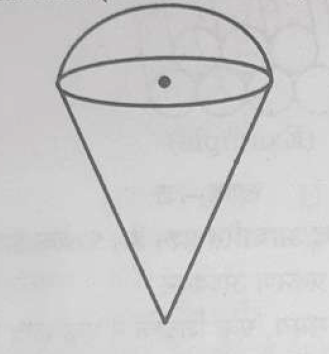
\includegraphics[width=\columnwidth]{figs/fig8.png}
  \caption{}
    \label{fig:figure3}
\end{figure}
\item If a line is drawn parallel to one side of a triangle to intersect the other two sides at distinct points, prove that the other two sides are divided in the same ratio.
\item The angle of elevation of the top of a tower $24$ m high from the foot of another tower in the same plane is ${60}{\degree}$. The angle of elevation of the top of second tower from the foot of the first tower is ${30}{\degree}$. Find the distance between two towers and the height of the other tower. Also, find the length of the wire attached to the tops of both the towers.
\item A spherical balloon of radius $r$ subtends an angle of ${60}{\degree}$ at the eye of an observer. If the angle of elevation of its centre is ${45}{\degree}$ from the same point, then prove that height of the centre of the balloon is $\sqrt{2}$ times its radius.
\item A chord of a circle of radius $14$ cm subtends an angle of ${60}{\degree}$ at the centre. Find the area of the corresponding minor segment of the circle. Also find the area of the major segment of the circle.
\item  If a pole $6 m$ high casts a shadow $2\sqrt{3}$  long on the ground,then sun's elevation is:
    \begin{enumerate}[label=(\alph*)]
        \item  $60\degree$
        \item  $45\degree$
        \item  $30\degree$
        \item  $90\degree$
    \end{enumerate}
    \item  In the given \figref{fig:figure2},$\triangle ABC \sim  \triangle QPR$.If $AC= 6 cm$,$BC = 5 cm$, $QR = 3 cm$ and $PR=x$;then the value of $x$is:
        \begin{enumerate}[label=(\alph*)]
            \item  $3.6 cm$
            \item  $2.5 cm$
            \item  $10 cm$
            \item  $3.2 cm$
               \begin{figure}[H]
  \centering
  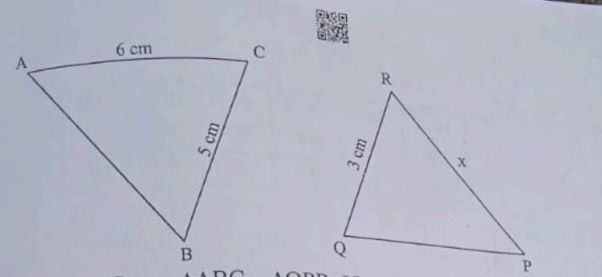
\includegraphics[width=\columnwidth]{figs/triangles.jpeg}
  \caption{}
  \label{fig:figure2}
\end{figure}
        \end{enumerate}
        \pagebreak
    \item  What is the area of a semi-circle of diameter $\lq d \rq$?
    \begin{enumerate}[label=(\alph*)]
        \item  $\frac{1}{16}\pi d^2$
        \item  $\frac{1}{4} \pi d^2$
        \item  $\frac{1}{8}\pi d^2$
        \item  $\frac{1}{2}\pi d^2$
    \end{enumerate}
    \item  In the given \figref{fig:figure1},$PQ \parallel AC$.If $BP = 4 cm$,$AP = 2.4 cm$ and $BQ = 5 cm$,then length of $BC$ is:
    \begin{enumerate}[label=(\alph*)]
        \item $8 cm$
        \item $3 cm$
        \item $0.3 cm$
        \item $\frac{25}{3}cm$
          \begin{figure}[H]
  \centering
  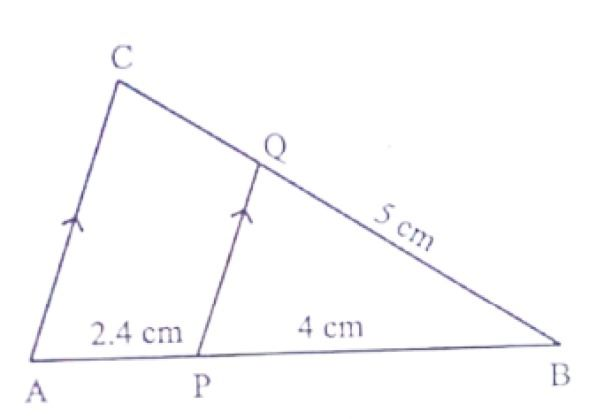
\includegraphics[width=\columnwidth]{figs/right angle triangle.jpeg}
  \caption{}
  \label{fig:figure1}
\end{figure}
    \end{enumerate}
    \pagebreak
       \item  In a $\triangle$  $PQR$,$N$ is a point on $PR$, such that $QN \perp PR$.If $PN \times NR = QN^2$, prove that $\angle PQR = 90 \degree$.
    \item   In the given \figref{fig:figure3}, $\triangle$ $ABC$ and  $\triangle$ $DBC$ are on the same base $BC$ at $O$,prove that
    \begin{align}
         \frac{ar (\triangle  ABC)}{ar (\triangle DBC)} = \frac{AO}{DO}.
    \end{align}
     \begin{figure}[H]
  \centering
  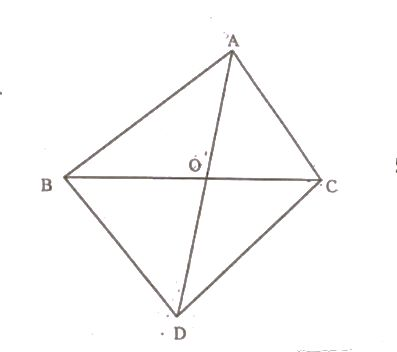
\includegraphics[width=\columnwidth]{figs/square.jpeg}
  \caption{}
  \label{fig:figure3}
\end{figure}
\pagebreak
     \item  A wooden article was made by scooping out a hemisphere from each end of a solid cylinder,as shown \figref{fig:figure4}.If the height of the cylinder is $10 cm$ and its base is of radius $3.5 cm$,find the total surface area of the article.
      \begin{figure}[H]
  \centering
  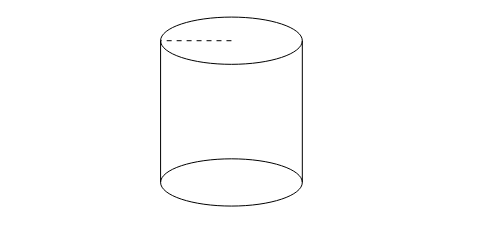
\includegraphics[width=\columnwidth]{figs/cylinder.png}
  \caption{}
  \label{fig:figure4}
\end{figure}


\end{enumerate}
%\end{document}











